% !TEX root = saveliev_physics_general_course_2.tex
%!TEX TS-program = pdflatex
%!TEX encoding = UTF-8 Unicode


\chapter[ELECTRIC CURRENT IN GASES]{ELECTRIC CURRENT
IN GASES}\label{chap:12}
\chaptermark{ELECTRIC CURRENT
IN GASES}

\section{Semi-Self-Sustained and Self-Sustained Conduction}\label{sec:12_1}

The passage of an electric current through gases is called a \textbf{gas discharge}.
Gases in their normal state are insulators, and current carriers are absent in them.
Only when special conditions are created in gases can current carriers appear in them (ions, electrons) and an electric discharge be produced.

Current carriers may appear in gases as a result of external action not associated with the presence of an electric field.
In this case, the gas is said to have \textbf{semi-self-sustained conduction}.
Semi-self-sustained discharge may be due to heating of a gas (thermal ionization), the action of ultraviolet rays or X-rays, and also to the action of radiation of radioactive substances.

If the current carriers appear as a result of processes due to an electric field being produced in a gas, the conduction is called \textbf{self-sustained}.
The nature of a gas discharge depends on many factors: on the chemical nature of the gas and electrodes, on the temperature and pressure of the gas, on the shape, dimensions, and mutual arrangement
of the electrodes, on the voltage applied to them, on the density and power of the current, etc.
This is why a gas discharge may have very diverse forms.
Some kinds of discharge are attended by a glow and sound effects---hissing, rustling, or crackling.

\section{Semi-Self-Sustained Gas Discharge}\label{sec:12_2}

Assume that a gas between electrodes (\fig{12_1}) continuously experiences a constant in intensity action of an ionizing agent (for example, X-rays).
The action of the ionizer results in one or more electrons being detached from some of the gas molecules.
The latter, thus, become positively charged ions.
At not very low pressures, the detached electrons are usually captured by neutral molecules, which, thus, become negatively charged ions.
Let $\Delta{\ab{n}{i}}$ stand for the number of pairs of ions appearing under the action of the ionizer in unit volume per second.

\begin{figure}[t]
	\begin{center}
		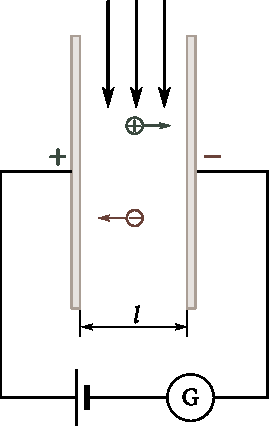
\includegraphics[scale=1]{figures/ch_12/fig_12_1.pdf}
		\caption[]{}
		\label{fig:12_1}
	\end{center}
	\vspace{-0.8cm}
\end{figure}

The process of ionization in a gas is attended by recombination of the ions, \ie, neutralization of unlike ions when they meet or the formation of a neutral molecule by a positive ion and an electron.

The probability of two ions of opposite signs meeting each other is proportional to the number of both positive and negative ions.
Hence, the number of pairs of ions $\Delta{\ab{n}{r}}$ recombining in unit volume per second is proportional to the square of the number of pairs of ions $n$ per unit volume:
\begin{equation}\label{eq:12_1}
    \Delta{\ab{n}{r}} = rn^2
\end{equation}

\noindent
($r$ is a constant of proportionality).

In a state of equilibrium, the number of appearing ions equals the number of recombining ones, hence,
\begin{equation}\label{eq:12_2}
    \Delta{\ab{n}{i}} = rn^2.
\end{equation}

\noindent
We, thus, get the following expression for the equilibrium concentration of ions (the number of pairs of ions in unit volume)·:
\begin{equation}\label{eq:12_3}
    n = \parenthesis{\frac{\Delta{\ab{n}{i}}}{r}}^{1/2}.
\end{equation}

Several pairs of ions appear per second in \SI{1}{\centi\metre} of atmospheric air under the action of cosmic radiation and traces of radioactive substances in the Earth's crust.
The constant $r$ for air is \SI{1.6e-6}{\centi\metre\cubed\per\second}.
Introduction of these values into \eqn{12_3} gives a value of about \SI{e3}{\centi\metre\cubed} for the equilibrium concentration of ions in the air.
This concentration is not adequate for the conduction to be noticeable.
Pure dry air is a very good insulator.

If we feed a voltage to electrodes, the ions will decrease in number not only because of recombination, but also because of the ions being drawn off by the field to the electrodes.
Assume that $\Delta{\ab{n}{j}}$ pairs of ions are drawn off from unit volume every second.
If the charge of each ion is $e'$, then the neutralization of one pair of ions on the electrodes is attended by the transfer of the charge $e'$ along the circuit.
Every second, $\Delta{\ab{n}{j}}Sl$ pairs of ions reach the electrodes (here, $S$ is the area of the electrodes, $l$ is the distance between them; the product $Sl$ equals the volume of the space between the electrodes).
Consequently, the current in the circuit is
\begin{equation*}
    I = e' \Delta{\ab{n}{j}} Sl,
\end{equation*}

\noindent
whence
\begin{equation}\label{eq:12_4}
    \Delta{\ab{n}{j}} = \frac{I}{e' l S} = \frac{j}{e' l},
\end{equation}

\noindent
where $j$ is the current density.

When a current is present, the condition of equilibrium is as follows:
\begin{equation*}
    \Delta{\ab{n}{i}} = \Delta{\ab{n}{r}} + \Delta{\ab{n}{j}}
\end{equation*}

\noindent
Substituting for $\Delta{\ab{n}{r}}$ and $\Delta{\ab{n}{j}}$ their values from \eqns{12_1}{12_4}, we arrive at the equation
\begin{equation}\label{eq:12_5}
    \Delta{\ab{n}{i}} = rn^2 + \frac{j}{e' l}.
\end{equation}

The current density is determined by the expression
\begin{equation}\label{eq:12_6}
    j = e' n \parenthesis{u_0^+ + u_0^-} E,
\end{equation}

\noindent
where $u_0^+$ and $u_0^-$ are the mobilities of the positive and negative ions, respectively [see \eqn{11_17}].

Let us consider two extreme cases---weak and strong fields.

With weak fields, the current density will be very small, and the addend $j/(e'l)$ in \eqn{12_5} may be disregarded in comparison with $rn^2$ (this signifies that the ions leave the space between the electrodes mainly as a result of recombination).
Equation \eqref{eq:12_5} thus transforms into \eqn{12_2}, and we get \eqn{12_3} for the equilibrium concentration of the ions.
Using this value of $n$ in \eqn{12_6}, we get
\begin{equation}\label{eq:12_7}
    j = e' \parenthesis{\frac{\Delta{\ab{n}{i}}}{r}}^{1/2} \parenthesis{u_0^+ + u_0^-} E.
\end{equation}

\noindent
The multiplier of $E$ in \eqn{12_7} does not depend on the field strength.
Hence, with weak fields, a semi-self-sustained gas discharge obeys Ohm's law.

The mobility of ions in gases has a value of the order of \SI{e-4}{\metre\squared\per\volt\per\second} [or \SI{1}{\centi\metre\squared\per\volt\per\second}]. Hence, at the equilibrium $n = \SI{e3}{\per\centi\metre\cubed} = \SI{e9}{\per\metre\cubed}$, and the field strength $E = \SI{1}{\volt\per\metre}$, the current density will be
\begin{equation*}
    j = \num{1.6e-19} \times \num{e9} \parenthesis{\num{e-4}+\num{e-4}} \times 1 \sim \SI{e-14}{\ampere\per\metre\squared} = \SI{e-18}{\ampere\per\centi\metre\squared}
\end{equation*}

\noindent
[see \eqn{12_6}; the ions are assumed to be singly charged].

With strong fields, we may disregard the addend $rn^2$ in \eqn{12_5} in comparison with $j/e'l$.
This signifies that virtually all the appearing ions will reach the electrodes without having time to recombine.
In these conditions, \eqn{12_5} becomes
\begin{equation*}
    \Delta{\ab{n}{i}} = \frac{j}{e' l},
\end{equation*}

\noindent
whence
\begin{equation}\label{eq:12_8}
    j = e' \Delta{\ab{n}{i}} l.
\end{equation}

\noindent
This current density is produced by all the ions originated by the ionizer in a column of the gas with unit cross-sectional area between the electrodes.
Consequently, this current density is the greatest at the given intensity of the ionizer and the given distance $l$ between the electrodes.
It is called the saturation current density $\ab{j}{sat}$.

Let us calculate $\ab{j}{sat}$ for the following conditions: $\Delta{\ab{n}{i}} = \SI{e-3}{\per\centi\metre\cubed}$ (this is approximately the rate of ion formation in the atmospheric air in ordinary conditions), $l = \SI{0.1}{\metre}$.
The introduction of these data into \eqn{12_8} yields
\begin{equation*}
    \ab{j}{sat} = \num{1.6e-19} \times \num{e7} \times \num{e1} \sim \SI{e-13}{\ampere\per\metre\squared} = \SI{e-17}{\ampere\per\centi\metre\squared}.
\end{equation*}

\noindent
These calculations show that the conduction of air in ordinary conditions is negligibly small.

\begin{figure}[t]
	\begin{center}
		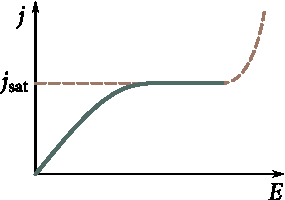
\includegraphics[scale=1]{figures/ch_12/fig_12_2.pdf}
		\caption[]{}
		\label{fig:12_2}
	\end{center}
	\vspace{-0.8cm}
\end{figure}

At intermediate values of $E$, there is a smooth transition from a linear dependence of $j$ on $E$ to saturation; when the latter is reached, $j$ stops depending on $E$ (see the solid curve in \fig{12_2}).
The region of saturation is followed by a region of a sharp growth in the current (see the portion of the curve depicted by the dash line).
The explanation of this growth is that beginning from a certain value of $E$, the electrons\footnote{Owing to the greater length of their free path, electrons acquire the ability to produce ionization by a collision earlier than gas ions do.} given birth to by the external ionizer manage to acquire a considerable energy while on their free path.
This energy is sufficient to ionize the molecules they collide with.
The free electrons produced in this ionization, after gaining speed, cause ionization in their turn.
Thus, an avalanche-like reproduction of the primary ions produced by the external ionizer occurs, and the discharge current is amplified.
The process does not lose its nature of a semi-self-
sustained discharge, however, because after the action of the external ionizer stops, the discharge continues only until all the electrons (primary and secondary) reach the anode (the rear boundary of the space containing ionizing particles---electrons---moves toward the anode).
For a discharge to become self-sustained, two meeting avalanches of ions are needed.
This is possible only if ionization by a collision is capable of giving birth to carriers of both signs.

It is very important that the semi-self-sustained discharge currents amplified as a result of reproduction of the carriers are proportional to the number of primary ions produced by the external ionizer.
This property of a discharge is used in proportional counters (see the following section).

\section{Ionization Chambers and Counters}\label{sec:12_3}

Ionization chambers and counters are employed for detecting and counting elementary particles, and also for measuring the intensity of X-rays and gamma rays.
The functioning of these instruments is based on the use of a semi-self-sustained gas discharge.

\begin{figure}[t]
	\begin{center}
		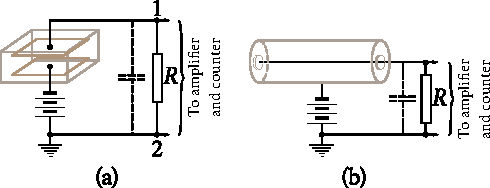
\includegraphics[scale=1]{figures/ch_12/fig_12_3.pdf}
		\caption[]{}
		\label{fig:12_3}
	\end{center}
	\vspace{-0.8cm}
\end{figure}

The schematic diagram of an ionization chamber and a counter is the same (\fig{12_3}).
They differ only in their operating conditions and structural features.
A counter (\fig{12_3}b) consists of a cylindrical body along whose axis a thin wire (anode) fastened on insulators is stretched.
The body of the counter is the cathode.
A window of mica or aluminium foil is made in the end of the counter to admit the ionizing particles.
Some particles, and also X-rays and gamma rays penetrate into a counter or an ionization chamber directly through their walls.
An ionization chamber (\fig{12_3}b) can have electrodes of various shapes.
In particular, they may be the same as in a counter, have the shape of plane parallel plates, etc.

Assume that a high-speed charged particle producing $N_0$ pairs of primary ions (electrons and positive ions) flies into the space between the electrodes.
The ions produced are carried along by the field toward the electrodes, and as a result a certain charge $q$, which we shall call a current pulse, passes through resistor $R$.
Figure \ref{fig:12_4} shows how the current pulse $q$ depends on the voltage $U$ between the electrodes for two different amounts of primary ions $N_0$ differing by three times ($N_{02} = 3N_{01}$).
Six regions can be earmarked on the graph.
Regions I and II were considered in the preceding section.
In particular, region II is the region of the saturation current---all the ions produced by an ionizing particle reach the electrodes without having
time to recombine.
It is quite natural that the current pulse does not depend on the voltage in these conditions.

Beginning from the value $\ab{U}{p}$, the field strength becomes sufficient for the electrons to be able to ionize the molecules by a collision. Therefore, the number of electrons and positive ions grows like an avalanche.
As a result, $AN_0$ ions reach each of the  electrodes.
The quantity $A$ is called the \textbf{gas amplification factor}.
In region III, this factor does not depend on the number of primary ions (but does depend on the voltage).
Therefore, if we keep the voltage constant, the current pulse will be proportional to the number of primary ions.
Region III is called the \textbf{proportional region}, and the voltage $\ab{U}{p}$ the \textbf{threshold of the proportional region}.
The gas amplification factor changes in this region from $1$ at its beginning to \num{e3}-\num{e4} at its end (the scale along the $q$-axis has not been observed in \fig{12_4}; only the ratio of $1$:$3$ between the ordinates in regions II and III has been
observed).

\begin{figure}[t]
	\begin{center}
		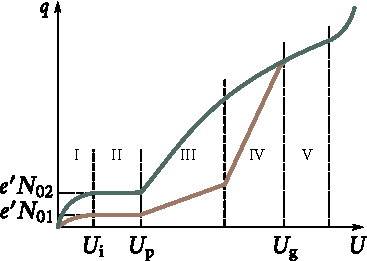
\includegraphics[scale=1]{figures/ch_12/fig_12_4.pdf}
		\caption[]{}
		\label{fig:12_4}
	\end{center}
	\vspace{-0.8cm}
\end{figure}

In region IV, called the \textbf{region of partial proportionality}, the gas amplification factor $A$ depends to a greater and greater extent on $N_0$.
In this connection, the difference between the current pulses produced by different numbers of primary ions becomes smoothed out more and more.

At voltages corresponding to region V (it is known as the \textbf{Geiger region}, and the voltage $\ab{U}{g}$ as the threshold of this region), the process acquires the nature of a self-sustained discharge.
The primary ions only produce an impetus for its appearance.
The current pulse in this region is absolutely independent of the number of primary ions.

In region VI, the voltage is so high that a discharge, after once being set up, does not stop.
It is, therefore, called the \textbf{region of continuous discharge}.

\textbf{Ionization Chambers.} An ionization chamber is an instrument operating without gas amplification, \ie, at voltages corresponding to region II.
There are two kinds of ionization chambers.
Chambers of one kind are used for registering the pulses initiated by individual particles (pulse chambers).
A particle flying into the chamber produces a certain number of ions in it, and as a result the current $I$ begins to flow through resistor $R$.
The result is that the potential of point $1$ (see \fig{12_3}a) rises and becomes equal to $IR$ (the initial potential of this point was the same as that of earthed point $2$).
This potential is fed to an amplifier, and after being amplified operates a counting device.
After all the charges that have reached the inner electrode pass through resistor $R$, the current stops and the potential of point $1$ again becomes equal to zero.
The nature of operation of the chamber depends on the duration of the current pulse set up by one ionizing particle.

\begin{figure}[t]
	\begin{center}
		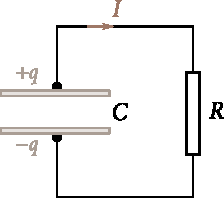
\includegraphics[scale=1]{figures/ch_12/fig_12_5.pdf}
		\caption[]{}
		\label{fig:12_5}
	\end{center}
	\vspace{-0.8cm}
\end{figure}

To determine what the duration of a pulse depends on, let us consider a circuit consisting of capacitor $C$ and resistor $R$ (\fig{12_5}).
If we impart the opposite charges $+q$ and $-q$ to the capacitor plates, a current will flow through resistor $R$, and the charges on the plates will diminish.
The instantaneous value of the voltage applied across the resistor is $U=q/C$.
Hence, we get the following expression for the current:
\begin{equation}\label{eq:12_9}
    I = \frac{U}{R} = \frac{q}{RC}.
\end{equation}

\noindent
Let us substitute $-\diffin{q}{t}$ for the current, where $-\deriv{q}$ is the decrement of the charge on the plates during the time $\deriv{t}$.
As a result, we get the differential equation
\begin{equation*}
    -\diff{q}{t} = \frac{q}{RC}\quad \text{or} \quad \frac{\deriv{q}}{q} = -\frac{q}{RC}\, \deriv{t}.
\end{equation*}

\noindent
According to \eqn{12_9}, $\deriv{q}/q=\deriv{I}/I$.
We can, therefore, write
\begin{equation*}
    \frac{\deriv{I}}{I} = - \frac{1}{RC}\, \deriv{t}.
\end{equation*}

\noindent
Integration of this equation yields
\begin{equation*}
    \ln{I} = - \frac{1}{RC}\, t + \ln{I_0}
\end{equation*}

\noindent
($\ln{I_0}$ is the integration constant).
Finally, raising the expression obtained to a power, we arrive at the equation
\begin{equation}\label{eq:12_10}
    I = I_0\, \exp\parenthesis{- \frac{t}{RC}}.
\end{equation}

\noindent
It is easy to see that $I_0$ is the initial value of the current.

It follows from \eqn{12_10} that during the time
\begin{equation}\label{eq:12_11}
    \tau = RC,
\end{equation}

\noindent
the current diminishes to $1/e$ of its original value.
Accordingly, the quantity $\tau$ is called the \textbf{time constant} of a circuit.
The greater this quantity, the slower is the rate of diminishing of the current in a circuit.

The diagram of an ionization chamber (see \fig{12_3}a) is similar to that shown in \fig{12_5}.
The part of $C$ is played by the interelectrode capacitance shown by a dash line on the diagram of the chamber.
An increase in the resistance of $R$ is attended by a growth in the voltage across points $1$ and $2$ at a given current, and this, consequently, facilitates the registration of the pulses.
This circumstance induces designers to use the highest possible resistance of $R$.
At the same time, for the chamber to be able to register separately the current pulses set up by particles rapidly following one another, the time constant must not be great.
Therefore, designers have to make a compromise when choosing the resistance of $R$ for pulse chambers.
It is usually taken of the order of \SI{e8}{\ohm}.
Hence, at $C\sim\SI{e-11}{\faraday}$, the time constant is \SI{e-3}{\second}.

Another kind of ionization chamber is the so-called integrating chamber.
The resistance of $R$ in them is of the order of \SI{e15}{\ohm}.
At $C\sim\SI{e-11}{\faraday}$, the time constant is \SI{e4}{\second}.
In this case, the current pulses produced by separate ionizing particles merge and a steady
current flows through the resistor.
Its magnitude characterizes the total charge of the ions produced in the chamber in unit time.
Thus, the ionization chambers of these two kinds differ only in the value of the time constant $RC$.

\textbf{Proportional Counters.} The pulses set up by separate particles can be amplified quite considerably (up to \num{e3}-\num{e4} times) if the voltage between the electrodes is in region III (see \fig{12_4}).
An instrument operating in such conditions is called a \textbf{proportional counter}.
The anode of the counter is made in the form of a wire of several hundredths of a millimetre in diameter.
The field strength near the wire is especially high.
With a sufficiently great voltage between the electrodes, the electrons produced near the wire acquire an energy under the action of the field that is adequate for producing ionization of the molecules by a collision.
The result is reproduction of the ions. The dimensions of the space in which reproduction occurs increase with the voltage. The gas amplification factor grows accordingly.

The number of primary ions depends on the nature and energy of the particles producing the pulse. Therefore, the magnitude of the pulses at the output of a proportional counter makes it possible to distinguish various particles, and also to sort particles of the same nature by their energies.

\textbf{Geiger-M\"uller Counters.} A still greater amplification of the pulse (up to \num{e8}) can be attained by making a counter function in the Geiger region (region V in \fig{12_4}).
A counter operating in these conditions is called a \textbf{Geiger-M\"uller counter} (or more briefly a \textbf{Geiger counter}).
A discharge in the Geiger region, being ``launched'' by an ionizing particle, subsequently transforms into a self-sustained one.
Hence, the magnitude of the pulse does not depend on the initial ionization.
To obtain separate pulses from individual particles, the discharge produced must be rapidly interrupted (quenched).
This is achieved either with the aid of an external resistance $R$ (in non-self-quenching counters), or at the expense of processes appearing in the counter itself.
In the latter case, the counter is called self quenching.

The quenching of a discharge with the aid of an external resistance is due to the fact that when a discharge current flows in the resistance, a great voltage drop is set up in it.
Consequently, only part of the applied voltage falls to the lot of the interelectrode space, and it is insufficient for maintaining the discharge.

Stopping of a discharge in self-quenching counters is due to the following reasons.
Electrons have a mobility that is about $1000$ times greater than the mobility of positive ions. Therefore, during the time it takes the electrons to reach the wire, the positive ions do not virtually move from their places.
These ions produce a positive space charge that weakens the field near the wire, and the discharge stops.
Quenching of the discharge in this case is prevented by additional processes which we shall not consider. To suppress them, an admixture of a polyatomic organic gas (for example, alcohol vapour) is added to the gas filling the counter (usually argon).
Such a counter separates pulses from particles following one another with an interval of the order of \SI{e4}{\second}.

\section[Processes Leading to the Appearance of Current Carriers]{Processes Leading to the Appearance of Current Carriers in a Self-Sustained Discharge}\label{sec:12_4}

Before commencing to describe the various kinds of self-sustained gas discharge, we shall consider the basic processes leading to the production of current carriers (electrons and ions) in such discharges.

\textbf{Collisions of Electrons with Molecules.} The collisions of electrons (and also ions) with molecules can have an elastic or inelastic nature.
The energy of a molecule (like that of an atom) is quantized.
This signifies that it can have only discrete (\ie, separated by finite intervals) values called energy levels.
The state with the smallest energy is called the \textbf{ground} one.
To transfer a molecule from its ground state to various excited ones, definite values of the energy $W_1$, $W_2$, etc., are needed.
A molecule can be ionized by imparting to it a sufficiently great energy $W_1$.

Upon transition to an excited state, a molecule usually stays in it only $\sim\SI{e-8}{\second}$, after which it passes back to its ground state, emitting its surplus energy in the form of a quantum of light---a \textbf{photon}.
Molecules can spend a considerably greater time (about \SI{e-3}{\second}) in certain excited states called \textbf{metastable}.

The laws of energy and momentum conservation must be obeyed when particles collide.
Therefore, definite limitations are imposed on the transfer of energy in a collision---not all the energy which a colliding particle has can be transferred to another particle.

If in a collision, an energy sufficient for exciting a molecule cannot be imparted to it, the total kinetic energy of the particles remains unchanged, and the collision will be \textbf{elastic}.
Let us find the energy imparted to the particle that is struck in an elastic collision.
Assume that a particle of mass $m_1$ having the velocity $v_{10}$ collides with a stationary ($v_{20}=0$) particle of mass $m_2$. The following conditions must be observed in a central collision:
\begin{align*}
    \frac{m_1v_{10}^2}{2} &= \frac{m_1v_1^2}{2} + \frac{m_2v_2^2}{2}\\
    m_1v_{10} &= m_1v_1 + m_2v_2,
\end{align*}

\noindent
where $v_1$ and $v_2$ are the velocities of the particles after the collision.
The velocity of the second particle from these equations will be
\begin{equation*}
    v_2 = \frac{2 m_1}{m_1 + m_2} v_{10}
\end{equation*}

\noindent
(see Sec. 3.11 of Vol. I).

The energy transmitted to the second particle in an elastic collision is determined by the expression
\begin{equation*}
    \Delta{\ab{W}{el}} = \frac{m_2v_2^2}{2} = \frac{m_1v_{10}^2}{2} \frac{4 m_1 m_2}{\parenthesis{m_1 + m_2}^2}.
\end{equation*}

\noindent
If $m_1\ll m_2$, this equation is simplified as follows:
\begin{equation}\label{eq:12_12}
    \Delta{\ab{W}{el}} = \frac{m_1v_{10}^2}{2} \frac{4 m_1}{m_2} = W_{10}\frac{4 m_1}{m_2}
\end{equation}

\noindent
where $W_{10}$ is the initial energy of the incident particle.

It can be seen from \eqn{12_12} that a light particle (electron) in an elastic collision with a heavy particle (molecule) gives up to it only a small fraction of its stock of energy.
The light particle ``rebounds'' from the heavy one like a ball from a wall, and its velocity remains virtually unchanged in magnitude.
The relevant calculations show that in a non-central collision the fraction of the energy transferred is still smaller.

With a sufficiently high energy of the incident particle (electron or ion), a molecule may be excited or ionized.
In this case, the total kinetic energy of the particles is not conserved---part of the energy goes for excitation or ionization, \ie, for increasing the internal energy of the colliding particles or for splitting one of the particles into two fragments.

Collisions attended by the excitation of particles are called in \textbf{elastic collisions of the first kind}.
A molecule in an excited state upon colliding with another particle (electron, ion, or neutral molecule) can pass over to the ground state without emitting its surplus energy, but transferring it to this particle.
As a result, the total kinetic energy of the particles after the collision will be greater than before it.
Such collisions are known as \textbf{inelastic collisions of the second kind}.
Molecules pass over from a metastable state to the ground one as a result of collisions of the second kind.

In an inelastic collision of the first kind, the equations of energy and momentum conservation have the form
\begin{align}
    \frac{m_1 v_{10}^2}{2} &= \frac{m_1 v_1^2}{2} + \frac{m_2 v_2^2}{2} + \Delta{\ab{W}{int}}, \label{eq:12_13}\\
    m_1 v_{10} &= m_1 v_1 + m_2 v_2,
\end{align}

\noindent
where $\Delta{\ab{W}{int}}$ is the increment of the internal energy of a molecule corresponding to its transition to an excited state.
Deleting $v_1$ from these equations, we get
\begin{equation}\label{eq:12_14}
    \Delta{\ab{W}{int}} = m_2 v_{10} v_2 - \parenthesis{\frac{m_1 + m_2}{m_1}} \frac{m_2v_2^2}{2}.
\end{equation}

At a given velocity of the striking particle ($v_{10}$), the increment of the internal energy $\Delta{\ab{W}{int}}$ depends on the velocity $v_2$ with which the molecule travels after the collision.
Let us find the greatest possible value of $\Delta{\ab{W}{int}}$.
To do this, we shall differentiate function \eqref{eq:12_14} with respect to $v_2$ and equate the derivative to zero:
\begin{equation*}
    \diff{\parenthesis{\Delta{\ab{W}{int}}}}{v_2} = m_2 v_{10} - \parenthesis{\frac{m_1 + m_2}{m_1}} m_2v_2 = 0.
\end{equation*}

\noindent
Hence, $_2 = m_1v_{10}/(m_1+m_2)$.
Substitution of this value for $v_2$ in \eqn{12_14} yields
\begin{equation}\label{eq:12_15}
    \Delta{\ab{W}{int,max}} = \parenthesis{\frac{m_2}{m_1+m_2}} \frac{m_1v_1^2}{2}.
\end{equation}

If the incident particle is considerably lighter than the struck one ($m_1\ll m_2$), the factor $m_2/(m_1+m_2)$ in \eqn{12_15} is close to unity.
Thus, when a light particle (electron) strikes a heavy one (molecule), almost all the energy of the incident particle can be used to excite or ionize the molecule\footnote{When ionization occurs, Eqs. \eqref{eq:12_13} become more complicated because there will be three particles instead of two after a collision. The conclusion on the possibility of spending almost all of the electron's energy for ionization is correct, however.}.

Even if the energy of the incident particle (electron) is sufficiently great, however, a collision does not necessarily result in the excitation or ionization of a molecule.
These processes have definite probabilities depending on the energy (and, therefore, on the velocity) of the electron.
Figure \ref{fig:12_6} shows the approximate path followed by these probabilities.
The higher the velocity of the electron, the smaller is the duration of its interaction with the molecule near which it flies.
Hence, both probabilities rapidly reach a maximum, and then diminish with an increase in the energy of the electron.
Inspection of the figure shows that an electron having, for example, the energy $W'$ will cause ionization of a molecule with greater probability than its excitation.

\begin{figure}[t]
	\begin{center}
		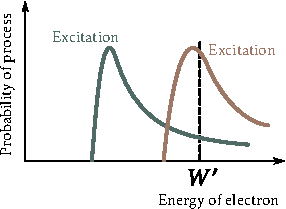
\includegraphics[scale=1]{figures/ch_12/fig_12_6.pdf}
		\caption[]{}
		\label{fig:12_6}
	\end{center}
	\vspace{-0.8cm}
\end{figure}

\textbf{Photoionization.} Electromagnetic radiation consists of elementary particles called \textbf{photons}.
The energy of a photon is $\hslash\omega$, where $\hslash$ is Planck's constant divided by $2\pi$ [see \eqn{7_43}], and $\omega$ is the cyclic frequency of the radiation.
A photon can be absorbed by a molecule, and its energy goes to excite or ionize the molecule.
In this case, the ionization of the molecule is called \textbf{photoionization}.
Ultraviolet radiation is capable of producing direct photoionization.
The energy of a photon of visible light is insufficient to detach an electron from a molecule.
Hence, visible radiation is not capable of producing direct photoionization.
It may be the cause, however, of so-called \textbf{stepped photoionization}.
This process is carried out in two steps.
In the first one, a photon transfers the molecule to
an excited state.
In the second step, the excited molecule is ionized as a result of its colliding with another molecule.

Short-wave radiation may appear in a gas discharge that is capable of producing direct photoionization.
A sufficiently fast electron may not only ionize a molecule when it collides with it, but also transfer the ion formed into an excited state.
The transition of an ion to the ground state is attended by the emission of radiation having a higher frequency than that of a neutral molecule.
The energy of a photon of such radiation is sufficient for direct photoionization.

\textbf{Emission of Electrons by the Surface of Electrodes.} Electrons may be supplied to a gas-discharge space as a result of their emission by the surface of the electrodes.
Such kinds of emission as thermionic (thermoelectron), secondary electron, and autoelectronic emission play the main part in some kinds of discharge.

\textbf{Thermionic emission} is the name given to the emission of electrons by heated solid or liquid bodies.
Owing to the free electrons in a metal having a variety of velocities in accordance with a distribution law, there is always a certain number of them whose energy is sufficient for them to overcome the potential barrier and leave the metal.
The number of such electrons at room temperature is negligibly small.
With elevation of the temperature, however, the number of electrons capable of leaving the metal grows very rapidly and becomes quite noticeable at a temperature of the order of \SI{1000}{\kelvin}.

By \textbf{secondary electron emission} is meant the emission of electrons by the surface of a solid or a liquid body when it is bombarded with electrons or ions.
The ratio of the number of emitted (secondary) electrons to the number of particles producing the emission is called the secondary electron emission coefficient.
When electrons are used to bombard the surface of a metal, the values of this coefficient vary from $0.5$ (for beryllium) to $1.8$ (for platinum).

\textbf{Autoelectronic} (or \textbf{cold}) \textbf{emission} is the emission of electrons by the surface of a metal occurring when an electric field of a very high strength ($\sim\SI{e8}{\volt\per\metre}$) is set up near the surface.
This phenomenon is also sometimes called field induced electron emission.

\section{Gas-Discharge Plasma}\label{sec:12_5}

Some kinds of self-sustained discharge are characterized by a very high degree of ionization.
A highly ionized gas, provided that the total charge of the electrons and ions in each elementary volume
equals (or almost equals) zero, is called a \textbf{plasma}.
A plasma is a special state of a substance.
The matter in the interior of the Sun and other stars having a temperature of scores of millions of kelvins is in this state.
A plasma produced owing to the high temperature of a substance is called \textbf{high-temperature} (or \textbf{isothermal}).
A \textbf{gas-discharge} plasma, as its name implies, is one produced in a gas discharge.

For a plasma to be in a stationary state, processes are needed that replenish the stock of ions diminishing as a result of recombination.
In high-temperature plasma, this is achieved as a result of thermal ionization, in gas-discharge plasma, as a result of collision ionization by electrons accelerated by an electric field.
The ionosphere (one of the layers of the atmosphere) is a special variety of plasma.
The high degree of ionization of the molecules ($\sim 1\%$) is maintained in the ionosphere by photoionization due to the Sun's shortwave radiation.

The electrons in a gas-discharge plasma participate in two motions---chaotic with a certain average velocity $\average{v}$ and ordered motion in a direction opposite to $\vec{E}$ with the average velocity $\average{u}$ much smaller than $\average{v}$.

\begin{figure}[t]
	\begin{center}
		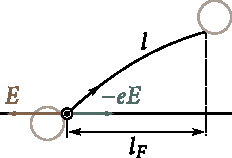
\includegraphics[scale=1]{figures/ch_12/fig_12_7.pdf}
		\caption[]{}
		\label{fig:12_7}
	\end{center}
	\vspace{-0.8cm}
\end{figure}

We shall prove that an electric field not only leads to ordered motion of the electrons of a plasma, but also increases the velocity $\average{v}$ of their chaotic motion.
Assume that at the moment when the field is switched on the gas contains a certain number of electrons whose average velocity corresponds to the gas temperature $\ab{T}{g}(m\average{v}^2/2 = 3k\ab{T}{g}/2)$·
In the interval between two successive collisions with molecules, an electron covers on an average the path $l$ (\fig{12_7}; the trajectory of the electron is curved slightly under the action of the force $-eE$).
The work done by the field on the electron is
\begin{equation}\label{eq:12_16}
    A = e E l_F,
\end{equation}

\noindent
where $l_F$ is the projection of the electron's path onto the direction of the force exerted on it.
Owing to collisions with molecules, the direction of motion of the electron constantly changes chaotically.
The magnitude and sign of $l$, change accordingly.
This is why the work given by \eqn{12_16} for separate portions of the path varies in magnitude and changes in its sign.
On some sections, the field increases the energy of the electron, on others diminishes it.
If ordered motion of the electrons were absent, the average value of $l$, and, consequently, the work given by \eqn{12_16} would be zero.
The presence of ordered motion, however, leads to the average value of the work $A$ differing from zero; it is positive and equals
\begin{equation}\label{eq:12_17}
    \average{A} = e E \average{u} \tau = e E \average{u} \frac{1}{\average{v}},
\end{equation}

\noindent
where $\tau$ is the average time needed by the electrons to cover their free path ($\average{u}\ll\average{u}$).

Thus, a field on an average increases the energy of the electrons.
True, an electron upon colliding with a molecule gives up part of its energy to it.
But, as we have seen in the preceding section, the fraction $\delta$ of the energy transferred in an elastic collision is very small---it averages\footnote{According to \eqn{12_12}, in a central collision $\delta = 4(m/M)$. When the electron and the molecule only slightly touch each other, we have $\delta\approx 0$.} $\delta = 2(m/M)$ (here $m$ is the mass of an electron, and $M$ that of a molecule).

In a rarefied gas (in which $l$ is greater) and with a sufficiently great field strength $E$, the work $\average{A}$ [\eqn{12_17}] may exceed the energy $m\average{v^2}\average{\delta}/2$ transferred on an average to a molecule in each collision.
The result will be a growth in the energy of chaotic motion of the electrons.
It ultimately reaches values sufficient to excite or ionize a molecule.
Beginning from this moment, part of the collisions stop being elastic and are attended by a large loss of energy.
Therefore, the average fraction $\average{\delta}$ of energy transferred increases.

Thus, the electrons acquire the energy needed for ionization not during one interval between collisions, but gradually in the course of a number of them.
Ionization leads to the appearance of a large number of electrons and positive ions---a plasma is produced.

The energy of the electrons of a plasma is determined by the condition that the average value of the work done by the field on an electron during one interval between collisions equals the average value of the energy given up by the electron upon colliding with a molecule:
\begin{equation*}
    e E \average{u} \frac{1}{\average{v}} = \frac{m \average{v^2}}{2} \average{\delta}.
\end{equation*}

\noindent
Here, $\delta$ is an intricate function of $\average{v}$.

Experiments show that the Maxwell distribution by velocities holds for the electrons in a gas-discharge plasma.
Owing to the weak interaction of the electrons with the molecules (in an elastic collision $\delta$ is very small, while the relative number of inelastic collisions is negligible), the average velocity of chaotic motion of the electrons is many times greater than the velocity corresponding to the temperature $\ab{T}{g}$ of the gas.
If we introduce the temperature of the electrons $\ab{T}{g}$ determining it from the equation $m\average{v^2}=3k\ab{T}{e}/2$, then we get a value of the order of several tens of thousands of kelvins for $\ab{T}{e}$.
The failure of the temperatures $\ab{T}{g}$ and $\ab{T}{e}$ to coincide indicates that there is no thermodynamic equilibrium between the electrons and molecules in a gas-discharge plasma\footnote{The average energy of the molecules, electrons, and ions in a high-temperature plasma is the same. This explains its other name---isothermal plasma.}.
The concentration of the current carriers in a plasma is very high.
Therefore, a plasma is an excellent conductor.
The mobility of the electrons is about three orders of magnitude greater than that of the ions.
Hence, the current in a plasma is mainly set up by its electrons.

\section{Glow Discharge}\label{sec:12_6}

A glow discharge appears at low pressures.
It can be observed in a glass tube about \SI{0.5}{\metre} long with flat metal electrodes soldered into its ends (\fig{12_8}).
A voltage of $\sim\SI{1000}{\volt}$ is supplied to the electrodes.
There is virtually no current in the tube at atmospheric pressure.
If the pressure is lowered, then approximately at \SI{50}{\mmHg} a discharge appears in the form of a glowing sinuous thin cord connecting the anode and the cathode.
Lowering of the pressure is attended by thickening of the cord, and at about \SI{5}{\mmHg} the cord fills the entire cross section of the tube---a glow discharge sets in.
Its principal parts are shown in \fig{12_8}.
Near the cathode is a thin luminous layer called the \textbf{cathode luminous film}.
Between the cathode and the luminous film is the \textbf{Aston dark space}.
At the other side of the luminous film is a weakly luminous layer which by contrast appears to be dark and is accordingly known as the \textbf{cathode} (or \textbf{Crookes}) \textbf{dark space}.
This layer bounds on a luminous region called the \textbf{negative glow}.
All the above layers form the cathode part of the glow discharge.

\begin{figure}[t]
	\begin{center}
		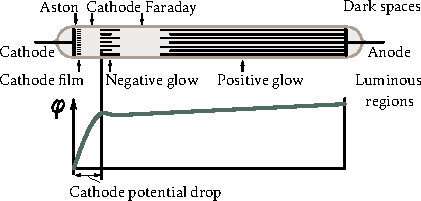
\includegraphics[scale=1]{figures/ch_12/fig_12_8.pdf}
		\caption[]{}
		\label{fig:12_8}
	\end{center}
	\vspace{-0.8cm}
\end{figure}

The negative glow is followed by the \textbf{Faraday dark space}.
The boundary between them is blurred.
The remaining part of the tube is filled with a luminous gas; it is called the \textbf{positive column}.
At a lower pressure, the cathode part of the discharge and the Faraday dark space become wider, while the positive column becomes shorter.
At a pressure of the order of \SI{1}{\mmHg}, the positive column breaks up into a number of alternating dark and light bent layers-\textbf{strata}.

Measurements made with the aid of probes (thin wires soldered in at different points along the tube) and by other means have shown that the potential changes non-uniformly along a tube (see the graph in \fig{12_8}).
Virtually the entire potential drop falls to the share of the first three parts of the discharge up to the cathode dark space inclusively.
This portion of the voltage applied to a tube is called the \textbf{cathode potential drop}.
The potential remains unchanged in the region of the negative glow---here the field strength is zero. Finally, the potential gradually grows in the Faraday dark space and in the positive column.
Such a distribution of the potential is due to the formation in the cathode dark space of a positive space charge because of the increased concentration of the positive ions.

The main processes needed to maintain a glow discharge occur in its cathode part.
The other parts of the discharge are not significant, they may even be absent (with a small spacing of the electrodes or at a low pressure).
There are two main processes---secondary electron emission from the cathode produced by its bombardment with positive ions, and collision ionization of the gas molecules by electrons.

The positive ions accelerated by the cathode potential drop bombard the cathode and knock electrons out of it.
These electrons are accelerated by the electric field in the Aston dark space.
Acquiring sufficient energy, they begin to excite the gas molecules, owing to which the cathode luminous film appears.
The electrons that fly without any collisions into the region of the cathode dark space have a high energy, and as a result they ionize the molecules more frequently than they excite them (see the graphs in \fig{12_6}).
Thus, the intensity of glowing of the gas diminishes, but in return many electrons and positive ions appear.
The ions produced first have a very low velocity.
As a result, a positive space charge is formed in the cathode dark space.
This leads to redistribution of the potential along the tube and to the appearance of the cathode potential drop.

The electrons appearing in the cathode dark space penetrate into the negative glow region that is characterized by a high concentration of electrons and positive ions and by a total space charge close
to zero (a plasma).
Therefore, the field strength here is very low.
Owing to the high concentration of electrons and ions, an intensive recombination process goes on in the negative glow region.
It is attended by the emission of the energy liberated during this process. Thus,
the negative glow is mainly a glow of recombination.

The electrons and ions penetrate from the negative glow region into the Faraday dark space because of diffusion (there is no field on the boundary between these regions, but in return there is a high gradient of electron and ion concentration).
The lower concentration of the charged particles greatly diminishes the probability of recombination in the Faraday dark space.
This is why the latter space seems to be dark.

A field is already present in the Faraday dark space.
The electrons carried away by this field gradually accumulate energy so that the conditions needed for the existence of a plasma finally appear.
The positive column is a gas-discharge plasma.
It plays the part of a conductor joining the anode to the cathode parts of the discharge.
The glow of the positive column is mainly due to transitions of excited molecules to their ground state.
Molecules of different gases emit radiation of different wavelengths in such transitions.
Therefore, the glow of the positive column has a characteristic colour for each gas.
This circumstance is taken advantage of in glow tubes for manufacturing luminous inscriptions and advertisements.
These inscriptions are the positive column of a glow discharge.
Neon gas-discharge tubes produce a red glow, argon ones a bluish-green glow, etc.

If the electrode spacing is gradually diminished, the cathode part of the discharge remains unchanged whereas the length of the positive column diminishes until this column disappears completely.
Next, the Faraday dark space disappears, and the length of the negative glow begins to decrease, the position of the boundary of this glow with the cathode dark space remaining unchanged.
When the distance from the anode to this boundary becomes very small, the discharge stops.

If the pressure is gradually lowered, the cathode part of the discharge extends over a greater and greater part of the interelectrode space, and finally the cathode dark space extends over almost the entire tube.
The glow of the gas in this case stops being noticeable but in return the tube walls begin to glow with a greenish colour.
The majority of the electrons knocked out of the cathode and accelerated by the cathode potential drop reach the tube walls without colliding with molecules of the gas and cause the walls to glow upon
striking them.
For historical reasons, the stream of electrons emitted by the cathode of a gas-discharge tube at very low pressures was called \textbf{cathode rays}.
The glow produced by bombardment with fast electrons
is called \textbf{cathodoluminescence}.

If a narrow canal is made in the cathode of a gas-discharge tube, part of the positive ions penetrate into the space beyond the cathode and form a sharply bounded beam of ions called canal (or positive) rays.
Beams of positive ions were first obtained in exactly this way.

\section{Arc Discharge}\label{sec:12_7}

In 1802, the Russian physicist Vasili Petrov (1761-1834) discovered that when contacting carbon electrodes connected to a large galvanic battery are moved apart, a concentrated light flares up between
the electrodes.
When the electrodes are horizontal, the heated luminescent gas bends in the shape of an arc.
This is why the phenomenon discovered by Petrov was called an \textbf{electric arc}.
The current in the arc may reach enormous values (from \SIrange{e3}{e4}{\ampere}) at a voltage
of several scores of volts.

An arc discharge can proceed at both a low (of the order of several millimetres of mercury) and a high (up to $1000$ atmospheres) pressure.
The main processes maintaining the discharge are thermionic emission from the heated cathode surface and thermal ionization of the molecules due to the high temperature of the gas in the space between the electrodes.
Almost the entire interelectrode space is filled with a high-temperature plasma.
It is the conductor through which the electrons emitted by the cathode reach the anode.
The temperature of the plasma is about \SI{6000}{\kelvin}.
In a superhigh-pressure arc, the temperature of the plasma may reach \SI{10000}{\kelvin} (we remind our reader that the temperature of the Sun's surface is \SI{5800}{\kelvin}).
Owing to bombardment by positive ions, the cathode is heated to about \SI{3500}{\kelvin}.
The anode, bombarded by a powerful stream of electrons, is heated still more.
As a result, the anode intensively evaporates, and a depression---a crater---is formed on its surface.
The crater is the brightest place in an arc.

An arc discharge has a dropping volt-ampere characteristic (\fig{12_9}).
The explanation is that a current increase is attended by a growth in the thermionic emission from the cathode and in the degree of ionization of the gas-discharge space.
As a result, the resistance of this space diminishes at a greater rate than that of the current increase.

\begin{figure}[t]
	\begin{center}
		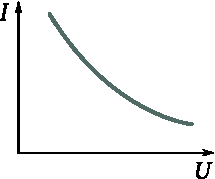
\includegraphics[scale=1]{figures/ch_12/fig_12_9.pdf}
		\caption[]{}
		\label{fig:12_9}
	\end{center}
	\vspace{-0.8cm}
\end{figure}

Apart from the thermionic arc described above (\ie, a discharge due to thermionic emission from the heated surface of the cathode) an \textbf{arc with a cold cathode} is also encountered.
Usually liquid mercury poured into a cylinder from which the air has been evacuated is the cathode of such an arc.
The discharge occurs in the mercury vapour.
The electrons fly out of the cathode as a result of autoelectronic emission.
The strong field at the cathode surface needed for this to occur is set up by the positive space charge formed by the ions.
The electrons are emitted not by the entire surface of the cathode, but by a small luminous and continuously moving cathode spot.
The temperature of the gas in this case is not high.
The molecules in the plasma are ionized, as in a glow discharge, as a result of collisions with the electrons.

\section{Spark and Corona Discharges}\label{sec:12_8}

A spark discharge is produced when the electric field strength reaches the breakdown value $\ab{E}{br}$ for the given gas.
The value of $\ab{E}{br}$ depends on the gas pressure; it is about \SI{3}{\mega\volt\per\metre}  (\SI{30}{\kilo\volt\per\centi\metre}) for air.
The value of $\ab{E}{br}$ varies with the pressure.
According to the experimentally established \textbf{Paschen law}, the ratio of the breakdown field strength to the pressure is approximately constant:
\begin{equation*}
    \frac{\ab{E}{br}}{p} \approx \text{constant}.
\end{equation*}

A spark discharge is attended by the formation of a brightly luminous tortuous branched canal along which a short-time strong current pulse flows.
An example is lightning; its length may be up to \SI{10}{\kilo\metre}, the diameter of the canal up to \SI{40}{\centi\metre}, the current may reach $100 000$ and more amperes, and the duration of the pulse is about \SI{e-4}{\second}.
Every stroke of lightning consists of several (up to $50$) pulses flowing along the same canal; their total duration (together with the intervals between the pulses) may reach several seconds.
The temperature of the gas in the spark canal is up to \SI{10000}{\kelvin}.
The rapid strong heating of the gas leads to a sharp growth in the pressure and the production of shock and sound waves.
This is why a spark discharge is attended by sound phenomena---from a weak crackling for a low-power spark to peals of thunder accompanying a stroke of lightning.

The appearance of a spark is preceded by the formation in the gas of a greatly ionized canal known as a streamer.
The latter is obtained by overlapping of the separate electron avalanches appearing along the path of the spark.
The forefather of each avalanche is an electron released by photoionization.
How a streamer develops is shown in \fig{12_10}.
Assume that the field strength has a value such that an electron flying out of the cathode as a result of some process or other acquires an energy sufficient for ionization along its free path.
This causes multiplication of the electrons to occur---an avalanche is formed (the positive ions appearing during this process do not play a noticeable part owing to their much smaller mobility; they only set up the space charge resulting in redistribution of the potential).
The short-wave radiation emitted by an atom that lost one of its inner electrons when ionized (this radiation is shown by wavy lines in the figure) produces photoionization of the molecules, the detached electrons giving birth to more and more new avalanches.
After overlapping of the avalanches, a well-conducting canal---a streamer---is formed along which a powerful stream of electrons flows from the cathode to the anode---breakdown occurs.

\begin{figure}[t]
	\begin{center}
		
\includegraphics[scale=1]{figures/ch_12/fig_12_10.pdf}
		\caption[]{}
		\label{fig:12_10}
	\end{center}
	\vspace{-0.8cm}
\end{figure}

If the electrodes have a shape at which the field in the space between them is approximately homogeneous (for example, they are spheres of a sufficiently great diameter), then breakdown occurs at a quite definite voltage $\ab{U}{br}$ whose value depends on the distance between the spheres $l$ ($\ab{U}{br} = \ab{E}{br}l$).
This underlies the design of a spark voltmeter used to measure high voltages (from \SIrange{e3}{e5}{\volt}).
During such measurements, the maximum distance $\ab{l}{max}$ is determined at which a spark appears.
Next multiplying $\ab{E}{br}$ by $\ab{l}{max}$, we get the value of the voltage being measured.

If one of the electrodes (or both) has a very great curvature (for example, the electrode is a thin wire or a sharp point), then when the voltage is not too high, a so-called \textbf{corona discharge} is produced.
When the voltage grows, this discharge transforms into a spark or an arc discharge.

In a corona discharge, the ionization and excitation of the molecules occur not in the entire interelectrode space, but only near an electrode having a small radius of curvature, where the field strength reaches values equal to or greater than $\ab{E}{br}$.
The gas glows in this part of the discharge.
The glow has the form of a corona surrounding the electrode, and this explains the name given to this kind of discharge.
A corona discharge from a point has the form of a luminous brush, and for this reason it is sometimes known as a \textbf{brush discharge}.
Positive and negative coronas are distinguished depending on the sign of the corona electrode.
The \textbf{external corona} region is between the corona layer and the non-corona electrode.
Breakdown conditions ($E\gg\ab{E}{br}$) exist only within the limits of the corona layer.
We can, therefore, say that a corona discharge is incomplete breakdown of the gas space.

With a negative corona, the phenomena at the cathode are similar to those at the cathode of a glow discharge.
The positive ions accelerated by the field knock electrons out of the cathode.
These electrons produce ionization and excitation of the molecules in the corona layer.
In the external region of the corona, the field is not sufficient to impart the energy needed for ionization or excitation of the molecules to the electrons.
For this reason, the electrons that penetrate into this region drift toward the anode under the action of the field.
Part of the electrons are captured by the molecules, the result being the formation of negative ions.
Thus, the current in the external region is due only to negative carriers-electrons and negative ions.
The discharge in this region is of a semi-self-sustained nature.

In a positive corona, the electron avalanches are conceived at the outer boundary of the corona and fly toward the corona electrodethe anode.
The appearance of electrons giving birth to avalanches is due to photoionization produced by the radiation of the corona layer.
The current carriers in the external region of the corona are the positive ions that drift to the cathode under the action of the field.

If both electrodes have a great curvature (two corona electrodes), processes occur near each of them that are characteristic of a corona electrode of the given sign.
Both corona layers are separated by an external region in which opposite streams of positive and negative current carriers travel.
Such a corona is called a bipolar one.

The self-sustained gas discharge mentioned in \sect{12_5} when treating counters is a corona discharge.

The thickness of the corona layer and the discharge current grow with an increasing voltage.
At a low voltage, the size of the corona is small, and its glow is hard to notice.
Such a microscopic corona is produced near a sharp point off which an electric wind flows (see
\sect{3_1}).

The bluish electrical glow caused by corona discharge on masts and other high parts of a ship at sea before and after electrical storms was called St. Elmo's fire in olden days.

In high-voltage facilities, for example, in high-tension transmission lines, a corona discharge leads to the harmful leakage of current.
Measures therefore have to be taken to prevent it.
For this purpose, for instance, the wires of high-tension lines are taken of a sufficiently large diameter, which is the greater, the higher is the voltage of the line.

The corona discharge has found a useful application in engineering in electrical filters.
The gas being purified flows through a tube along whose axis a negative corona electrode is arranged.
The negative ions present in a great number in the external region of the corona settle on the particles or droplets polluting the gas and are carried along with them to the external non-corona electrode.
Upon reaching the latter, the particles become neutralized and settle on it.
Later, blows are struck at the tube and the sediment formed by the precipitated particles drops into a collector.
